\documentclass{article}
\setcounter{tocdepth}{3}
\usepackage{setspace,graphicx,array}
\usepackage[utf8]{inputenc}
\usepackage[left=1in,top=1in,right=1in,bottom=1in]{geometry} % Document margins
\onehalfspacing

% Setting the depth for Table of Contents
\setcounter{tocdepth}{2}

\begin{document}

% --- TITLE PAGE ---
\title{Donnervögel Consulting \\ MarkShark Project Planning Document}
\author{Markus Balaski \\ Graeme Smith \\ Jordan Toering \\ Stephen Laboucane \\ Ian Pun \\ Colin Woodbury \\ Chazz Young}
\maketitle
\clearpage
% ------------------

% --- REVISION HISTORY ---
% Add more entries here as the Spec undergoes major changes.
% More recent entries come first.
\textbf{Revision History}
\begin{center}
  \begin{tabular}{| c | c | c | l |}
    \hline
    Version & Date & Members & Changes\\
    \hline
    1.0 & 2014 Feb 6 & Markus B. & Planning Document Created.\\
    & & Graeme S. & \\
    & & Jordan Toering & \\
    & & Stephen L. & \\
    & & Ian P. & \\
    & & Colin W. & \\
    & & Chazz Y. & \\
    \hline
  \end{tabular}
\end{center}
\clearpage
% -------------------------

% --- TABLE OF CONTENTS ---
\tableofcontents
\clearpage
% -------------------------

% --- BEGIN SECTIONS ---

\section{Project Overview}
This project is a prototype to demonstrate the feasibility of a grading system.
There will be users of this system: System Administrators, Academic Administrators,
Administrative Assistants, Instructors,  and TA/TM markers.\\
Roles:
\begin{itemize}
  \item System Administrator
   \begin{itemize}
     \item Responsible for the creation and management of accounts, program
       installation, and system backups/restores.
     \item Also manages the system log, which records all activities done by the
       grading system.
   \end{itemize}
   \item Academic Administrator
     \begin{itemize}
       \item Responsible for overseeing the grading system and changing grades
         in the case of a grade dispute, if necessary.
       \item Also manages the Academic Log, which records all grading changes
         in the system.
     \end{itemize}
   \item Administrative Assistant
     \begin{itemize}
       \item Responsible for the creation of courses (including the copying
         and deletion of courses)
     \end{itemize}
   \item Instructor
     \begin{itemize}
       \item Responsible for the creation of management of activities within
         the courses they are teaching.
       \item Responsible for the management of students, student groups, and
         assigning TAs to assignments and student groups.
       \item May also grade activities within their courses.
     \end{itemize}
   \item TA/TM
     \begin{itemize}
       \item Primary graders for the assignments and students assigned to them
         by the Instructor of the course.
     \end{itemize}
\end{itemize}

\section{Project Planning}
\subsection{Risk Management}
\subsubsection{External Library Issues}
The usage of any external libraries of code in our project presents a risk.\\
Scenario: Portions of the project that we might plan to use external libraries
for are not applicable or will not properly function in our project as
we expect.\\
Action Plan: An action plan to eliminate this risk is to minimise any reliance
on external libraries as much as possible. In addition to this, we can also
find multiple libraries that might work for any components requiring an external
library, so as to have backups in the case of any unforeseen incompatibilities
or issues.

\subsubsection{Client OS Change}
Scenario: Management has changed and decided to support a different OS.\\
Action Plan: To keep our budget low for our prototype, coding in java has many
benefits to creating something time efficient and also cross platform.
As such, it is important for our prototype to consider older java libraries
compared to newly updated ones so, in the case of where the client has changed
to a different OS with different java version support, it would be minimal
effort to convert our prototype to one that matches for our client.
\subsubsection{User Specification Change}
Scenario: The client has decided to change what a user will be allowed to do, e.g.
they want an Administrative Assistant to be able to grade as well.\\
Action Plan: An action plan to reduce the impact of this risk is to implement
tasks users can perform as modularly as possible. This will ease the addition or
removal of functions.

\subsubsection{Government/International Regulations Change}
Scenario: Powers greater than the client changed parameters of the project.\\
Contingency Plan: One way to recover from such an unexpected twist is to 
notify the client that circumstances have changed, which may or may not 
delay the final product.  Additionally, a small new team may be hired to 
make the necessary conversions instead of diverting core employees already 
working on the project, if the required changes are non-trivial and time is 
an important issue.  Else the standard management plan should have provided 
time and resources for minor hiccups, and they could be applied here.


\section{Meeting Documentation}
Compilation of Minutes and Agendas since January 20.  We had multiple meetings
 so total content is spread across four meetings.  All meetings start at 2:45 
 and conclude when we have worked through the agenda.

\subsection{January 20}
\begin{itemize}
\item Attendance: All members.
\item Room: TASC 9204E [Client Meeting]
\end{itemize}
\subsubsection{Agenda}
\begin{itemize}
\item Set up and test recording device.
\item Have each member present their questions to the client.
\item Notate important specifications that we may need to clarify later on in
 the meeting.
\end{itemize}
\subsubsection{Minutes}
\begin{itemize}
\item Microphone successfully set up and recording.
\item Each member presented their section and received clarification 
when necessary.
\item Transcription of recorded meeting was assigned to Graeme and Markus.
\end{itemize}

\subsection{January 24}
\begin{itemize}
\item Attendance: All members.
\item Room: 2007 Library
\end{itemize}
\subsubsection{Agenda}
\begin{itemize}
\item Review the Client Meeting Transcript.
\item Introduce LaTeX as a tool to create deliverables.
\item Start the Requirements Specification using LaTeX.
\end{itemize}
\subsubsection{Minutes}
\begin{itemize}
\item Members were reminded to push a picture of themselves to the images 
folder in the repository.
\item All of the members read and briefly discussed the transcribed 
client meeting.
\item Created the rough project specification file, added content and color 
coded the requirements in the specification file{using Google Docs}.
\item Jordan will email the CS office front desk requesting a room on behalf
 of the group.
\item Colin will create the LaTeX document skeleton, complete with 
format templates. Content can be added and pushed to
 the document through GitHub.
\item As a closing remark, we added the link to the Google Doc the useful
 links section for future reference. 
\item Ian volunteered a suggestion to use the meeting room in the SFU 
residences for the next meeting as they will be available and 
suitable to our needs.
\end{itemize}

\subsection{January 27}
\begin{itemize}
\item Attendance: All members.
\item Room: Shell House Social Room
\end{itemize}
\subsubsection{Agenda}
\begin{itemize}
\item Review our LaTeX document for organization and consistency between
 sections.
\item Inform members of suitable LaTeX editors and sort out any issues with
 viewing and editing the document on GitHub.
\end{itemize}
\subsubsection{Minutes}
\begin{itemize}
\item LaTeX document was reviewed and edited for consistency.
\item Members should acquire a development environment and finalize their 
content contributions by tonight so we can submit the assignment tomorrow.
\item Specified missing sections and assigned members to complete them.
\item Group was in favor of meeting in this room for next meeting.
\item Scheduled next meeting for this coming Friday to prepare further
 for next deliverable due date.
\end{itemize}

\subsection{January 31}
\begin{itemize}
\item Attendance: All members except Graeme.  He informed the group 
beforehand of his absence(due to cultural event) and made arrangements to 
be kept up to date with the events of the meeting.
\item Room: Shell House Social Room
\end{itemize}
\subsubsection{Agenda}
\begin{itemize}
\item Brainstorm and prepare questions for Feb. 3rd client 
requirements review meeting.
\item Finalize content addition responsibilities for Feb. 
3rd requirements review meeting.  
\item Create LaTeX document for next deliverable.
\end{itemize}
\subsubsection{Minutes}
\begin{itemize}
\item Group members reviewed the online criteria for the requirements 
review meeting.
\item A second Google Doc was created to assist with collaborative work 
on the preparation for the next group meeting.
\item Members will finalize their contributions to the second Google Doc 
and the final copy will be converted to Markdown for easy reading.
\item Markus will create LaTeX skeleton for the deliverable following the 
requirements review meeting.
\item Over the weekend, members should add their content to the Deliverable
 1 LaTeX document and ensure their scenarios for the client requirements 
 review meeting(Tuesday) are complete.
\end{itemize}

\section{Team Member Roles}
\begin{center}
\begin{tabular}{c c p{2in}}
  Member & Name & Info \\
  \hline
  {\raisebox{-.8\height}{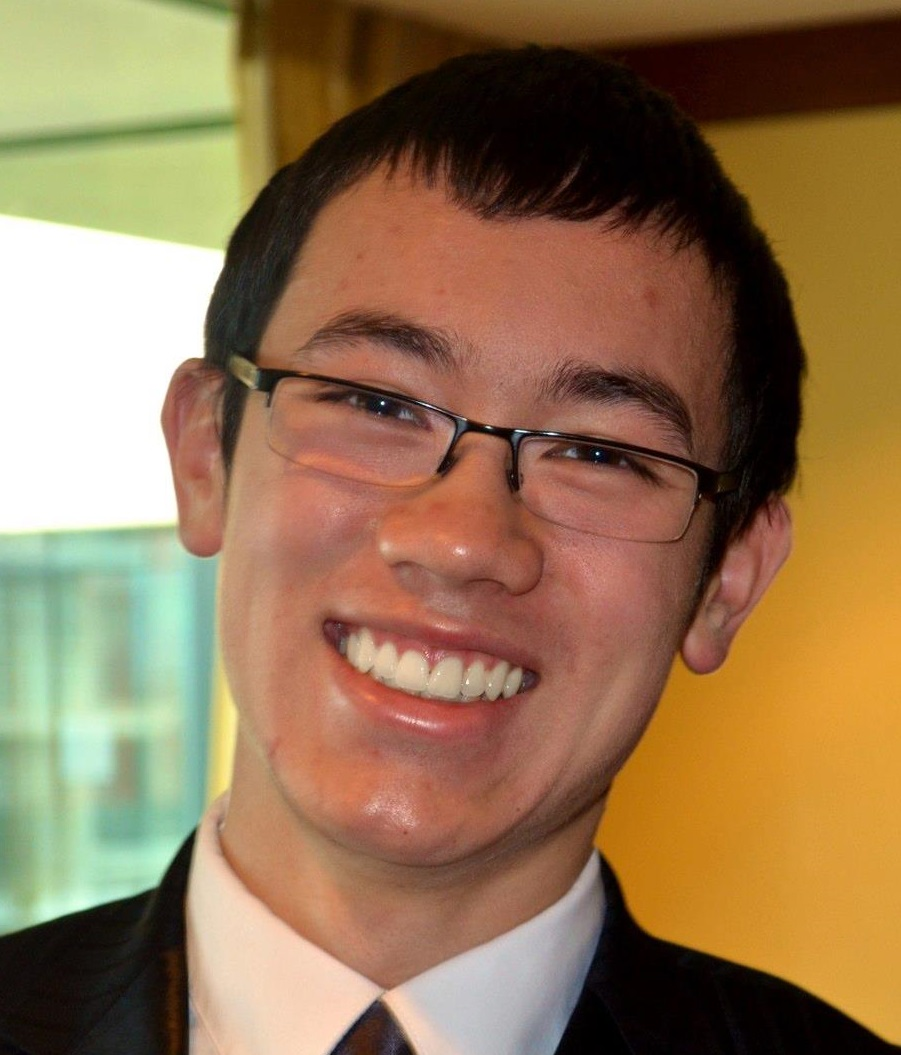
\includegraphics[scale=0.125]{../images/groupPhotos/Graeme}}}
  & Graeme Smith
  &
  \begin{itemize}
    \item gds3@sfu.ca
    \item Minutes Taker 2
    \item Phase 4 Leader
  \end{itemize} \\
  \hline
  {\raisebox{-.8\height}{
\includegraphics[scale=0.09]{../images/groupPhotos/Colin}}}
  & Colin Woodbury
  & \begin{itemize}
      \item cwoodbur@sfu.ca
      \item Configuration Manager 1
      \item Phase 5 Leader
    \end{itemize} \\
  \hline
  {\raisebox{-.8\height}{
\includegraphics[scale=0.05]{../images/groupPhotos/Stephen}}}
  & Stephen Laboucane
  & \begin{itemize}
      \item slabouca@sfu.ca
      \item Meeting Manager 2
      \item Phase 7 Leader
    \end{itemize} \\
  \hline
  {\raisebox{-.8\height}{
\includegraphics[scale=0.3]{../images/groupPhotos/Chazz}}}
  & Chazz Young
  & \begin{itemize}
      \item chazzy@sfu.ca
      \item Configuration Manager 2
      \item Phase 1 Leader
    \end{itemize} \\
  \hline
  {\raisebox{-.8\height}{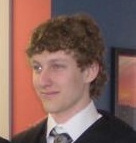
\includegraphics[scale=0.8]{../images/groupPhotos/Jordan}}}
  & Jordan Toering
  & \begin{itemize}
      \item jtoering@sfu.ca
      \item Minutes Taker 1
      \item Phase 2/9 Leader
    \end{itemize}
\end{tabular}
\end{center}

\begin{center}
\begin{tabular}{c c p{2in}}
  Member & Name & Info \\
  \hline
  {\raisebox{-.8\height}{
\includegraphics[scale=0.2]{../images/groupPhotos/MarkusB}}}
  & Markus Balaski
  & \begin{itemize}
      \item mabalaski@gmail.com
      \item Communications Manager
      \item Phase 3/8 Leader
    \end{itemize} \\
  \hline
  {\raisebox{-.8\height}{
\includegraphics[scale=0.45]{../images/groupPhotos/Ian}}}
  & Ian Pun
  & \begin{itemize}
      \item itpun@sfu.ca
      \item Meeting Manager 1
      \item Phase 6 Leader
    \end{itemize}
\end{tabular}
\end{center}

\end{document}
